\section{Extended Scenarios}
\label{sec:extended-scenarios}

The previous section reviewed reasoning segmentation in static images, where the target is inferred from implicit language, dialogue context, false premises, or domain rules before a mask is produced. This section studies extended scenarios. They are not merely new application domains. Each scenario changes one of the assumptions used by image-level open-vocabulary and reasoning segmentation: videos add time and tracking, 3D scenes add geometry and viewpoint dependence, remote-sensing imagery changes scale and domain language, medical imaging introduces clinical rules and modality-specific evidence, and affordance or embodied grounding asks for action-relevant regions rather than object categories.

Following the writing logic of this survey, we organize these extensions by the ambiguity they introduce. Table~\ref{tab:extended-scenario-index} summarizes representative resources, verified data or protocol facts from the original papers, and the core stress test of each scenario. The table is not intended as a leaderboard. Instead, it records what must be reported before comparisons in Section~\ref{sec:comparison-discussion} can be meaningful: modality, supervision unit, dataset scale, task protocol, metric family, and the source of reasoning or grounding cues. Evaluation limitations are discussed in the corresponding subsections.

\begin{table*}[t]
\centering
\small
\setlength{\tabcolsep}{4pt}
\renewcommand{\arraystretch}{1.20}
\caption{Representative extended scenarios for open-vocabulary, promptable, grounded, and reasoning segmentation. Dataset and protocol facts are taken from the cited papers rather than inferred from method names; detailed evaluation limitations are discussed in the corresponding subsections.}
\label{tab:extended-scenario-index}
\begin{tabularx}{\textwidth}{>{\raggedright\arraybackslash}p{0.16\textwidth}>{\raggedright\arraybackslash}X>{\raggedright\arraybackslash}p{0.34\textwidth}>{\raggedright\arraybackslash}p{0.26\textwidth}}
\toprule
Scenario & Representative tasks and methods & Verified data or protocol facts & Key stress test \\
\midrule
Video reasoning and grounded chat & VideoLISA~\citep{baiOneTokenSeg2024}; ViLLa~\citep{zhengVillaVideoReasoning2025}; VideoSeg-R1~\citep{xuVideosegr1ReasoningVideo2026}; SAMA~\citep{sunSamaMultiturnReferential2026}; VideoGLaMM~\citep{munasingheVideoglammLargeMultimodal2025}; ViCaS~\citep{atharVicasDatasetCombining2025} & ReasonVOS~\citep{baiOneTokenSeg2024}: 91 videos and 458 video-instruction-mask samples; VideoReasonSeg~\citep{zhengVillaVideoReasoning2025}: 3k videos and 15k object-instruction pairs; SAMA-239K~\citep{sunSamaMultiturnReferential2026}: 15,143 videos, 172,296 grounded video-QA triplets, and 67,005 captioning samples; SAMA-Bench~\citep{sunSamaMultiturnReferential2026}: 5,067 questions from 522 videos. & Tests temporal reasoning, key-frame or key-segment selection, mask propagation, multi-object occlusion, and grounded multi-turn dialogue. \\
Audio-visual and omnimodal video grounding & TGS-Agent~\citep{zhouThinkYouSegment2026}; AL-Ref-SAM2~\citep{huangUnleashingTemporalspatialReasoning2025}; OmniAVS/OISA~\citep{yingOmnimodalExpressionsReasoning2025}; Omni-R1~\citep{zhongOmnir1ReinforcementLearning2026} & Ref-AVSBench~\citep{zhouThinkYouSegment2026}: 4,000 10-second videos and 20,000 expressions; R2-AVSBench~\citep{zhouThinkYouSegment2026}: 400 rewritten test videos with reasoning-intensive references; OmniAVS~\citep{yingOmnimodalExpressionsReasoning2025}: 2,104 videos and 61,095 multimodal expressions. & Tests whether text, sound, speech, and visual evidence are aligned before the target is segmented. \\
3D and multiview grounding & 3D-DRES~\citep{chen3DDRESDetailed3D2026}; Surprise3D~\citep{huangSurprise3dDatasetSpatial2026}; OV3D~\citep{jianglOpenvocabulary3dSemantic2024}; SAI3D~\citep{yyinSai3dSegmentAny2024}; XMask3D~\citep{zwangXmask3dCrossmodalMask2024}; OV3D-CG~\citep{mzhouOV3DCGOpenvocabulary3D2025} & DetailRefer~\citep{chen3DDRESDetailed3D2026}: 54,432 descriptions over 11,054 objects and 2.9 masks per text on average; Surprise3D~\citep{huangSurprise3dDatasetSpatial2026}: more than 200k vision-language pairs across 900+ ScanNet++ scenes, with 89k+ human spatial queries and 2.8k+ object classes. & Tests phrase-to-instance mapping, viewpoint ambiguity, 2D-to-3D mask transfer, and spatial relations beyond object-name shortcuts. \\
Remote sensing and aerial imagery & OVRSISBench/RSKT-Seg~\citep{libExploringEfficientOpenvocabulary2026}; AerOSeg~\citep{sduttaAerosegHarnessingSam2025}; ZoRI~\citep{huangZoRIDiscriminativeZeroshot2025}; RIS-LAD~\citep{yeRISLADBenchmarkModel2026}; LISAt~\citep{quenumLisatLanguageinstructedSegmentation2026}; GeoChat~\citep{kuckrejaGeochatGroundedLarge2024} & OVRSISBench~\citep{libExploringEfficientOpenvocabulary2026}: 8 reformulated remote-sensing datasets with mIoU and mACC; RIS-LAD~\citep{yeRISLADBenchmarkModel2026}: 13,871 image-text-mask triplets from low-altitude drone imagery; LISAt/GRES~\citep{quenumLisatLanguageinstructedSegmentation2026}: 27,615 annotations over 9,205 images and PreGRES with over 1M QA pairs. & Tests small dense objects, rotation and viewpoint variation, land-cover vocabularies, cross-dataset transfer, and geospatial reasoning. \\
Medical grounding & MedReasoner~\citep{yanMedreasonerReinforcementLearning2026}; MIMO~\citep{chenMIMOMedicalVision2025}; medical pixel-grounded MLLMs & U-MRG-14K~\citep{yanMedreasonerReinforcementLearning2026}: 14K image-mask pairs with implicit clinical queries and reasoning traces across 10 modalities, 15 super-categories, and 108 categories. & Tests clinical inference before localization, modality-specific evidence, and guideline-like region definitions. \\
Affordance and embodied grounding & AffordanceLLM~\citep{qianAffordancellmGroundingAffordance2024}; Affordance-R1~\citep{wangAffordancer1ReinforcementLearning2026}; OpenHOI~\citep{zhangOpenhoiOpenworldHandobject2026}; instruction-guided visual masking~\citep{zhengInstructionguidedVisualMasking2024} & ReasonAff~\citep{wangAffordancer1ReinforcementLearning2026}: affordance-centric reasoning; Affordance-R1~\citep{wangAffordancer1ReinforcementLearning2026}: ReasonAff and AGD20K/UMD evaluation with gIoU, cIoU, P50-95, and P50; IVM-Mix~\citep{zhengInstructionguidedVisualMasking2024}: 1M image-instruction pairs. & Tests functional regions, action feasibility, part-level grounding, and open-world manipulation instructions. \\
\bottomrule
\end{tabularx}
\end{table*}

\subsection{Video reasoning and tracking-aware segmentation}

Video extensions expose the temporal side of reasoning segmentation. In image reasoning segmentation, a \texttt{<SEG>} token, mask proposal, or pixel decoder can be interpreted against one visual state. In videos, the same target may be visible, occluded, deformed, partially out of frame, or referred to by an event that unfolds over time. Therefore, the core question changes from ``which region matches this query'' to ``which temporally evolving object satisfies this query and how should its mask be propagated across frames.''

VideoLISA is the natural bridge from image-level LISA-style reasoning to videos. It introduces sparse dense sampling to balance long temporal context with high-resolution dense prediction, and uses a special \texttt{<TRK>} token so that one generated token can segment and track the same object across multiple frames~\citep{baiOneTokenSeg2024}. The associated ReasonVOS benchmark contains 91 videos and 458 video-instruction-mask samples, including short object descriptions and longer reasoning instructions. This is an important change in supervision: the unit is no longer a single image-query-mask triplet, but a video-instruction-mask sequence that tests temporal understanding, tracking consistency, and implicit target inference.



ViLLa makes the video-specific bottleneck more explicit. As indicated by the planned Fig.~\ref{fig:extended-villa-placeholder}, it does not only add a video encoder to an image model. It introduces a key segment extractor to reduce long-video redundancy, a context synthesizer to encode user intent with video context, and a hierarchical temporal synchronizer for local and global multi-object interactions~\citep{zhengVillaVideoReasoning2025}. Its VideoReasonSeg benchmark contains 3k videos and 15k object-instruction pairs, split across short and long videos and designed around complex scenarios such as multiple objects, rapid motion, and occlusion. VideoSeg-R1 then brings RL into the same setting by decomposing video reasoning segmentation into text-guided frame sampling, reasoning with spatial cues, and SAM2/XMem-based segmentation propagation~\citep{xuVideosegr1ReasoningVideo2026}. This mirrors the RL trend in Section~\ref{sec:reasoning-segmentation}, but the reward must now account for both target inference and temporal mask propagation.

Grounded video chat broadens the output interface. ViCaS and VideoGLaMM connect holistic video understanding with pixel-level grounded segmentation, while SAMA unifies video referring understanding, grounding, and multi-turn dialogue~\citep{atharVicasDatasetCombining2025,munasingheVideoglammLargeMultimodal2025,sunSamaMultiturnReferential2026}. SAMA-239K contains 15,143 videos, 172,296 referential grounded video-QA triplets, and 67,005 referential captioning samples; SAMA-Bench contains 5,067 questions from 522 videos. This data design shows why video grounding cannot be evaluated only as mask propagation. A model must also answer questions, keep dialogue referents stable, and ground generated object mentions in spatio-temporal masks.

\begin{figure*}[htbp]
    \centering
    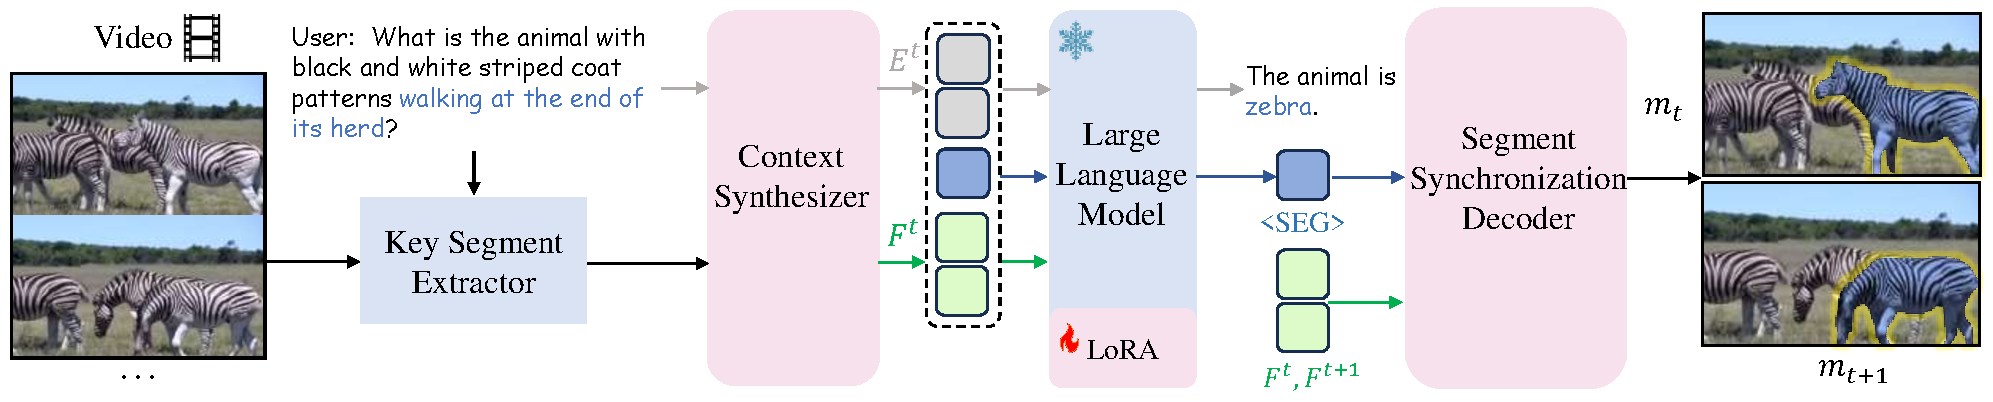
\includegraphics[width=1\textwidth]{Fig/fig_ViLLa.pdf}
    \caption{ViLLa's video reasoning segmentation framework. This placeholder should be replaced by the original overall framework figure from ViLLa, which shows the key segment extractor, context synthesizer, and hierarchical temporal synchronizer that connect user intent, selected video segments, and multi-scale segmentation tokens~\citep{zhengVillaVideoReasoning2025}.}
    \label{fig:extended-villa-placeholder}
\end{figure*}

The limitation of video methods is comparability. Standard referring video object segmentation often reports $\mathcal{J}$, $\mathcal{F}$, or $\mathcal{J}\&\mathcal{F}$, while grounded video chat adds mIoU, recall, and language-generation metrics. A model may improve temporal propagation with SAM2 memory~\citep{ravi2024sam2} while still reasoning over the wrong frame, or may answer a dialogue turn correctly while grounding the wrong track. For this reason, video reasoning segmentation should report frame sampling, prompt source, propagation module, target-selection evidence, and separate reasoning and mask metrics.



\subsection{Audio-visual and omnimodal grounding}

Audio-visual grounding adds another ambiguity: the reference may be auditory, linguistic, visual, or a combination of all three. Referring audio-visual segmentation asks the model to segment the object in an audible video according to a reference expression. The referred entity may be identified by what it sounds like, who interacts with it, or where the sound comes from. This makes simple text-to-box-to-mask composition brittle when the text names only an action or sound source.

TGS-Agent responds by decomposing the task into Think, Ground, and Segment. A multimodal language model first reasons over textual, visual, and auditory cues, produces an explicit object description, and then passes that description to Grounding DINO and SAM2 for localization and segmentation~\citep{zhouThinkYouSegment2026}. The original Ref-AVSBench has 4,000 10-second videos and 20,000 expressions, while R2-AVSBench rewrites 400 test videos with longer and more reasoning-intensive references. This benchmark construction is useful because it keeps the underlying masks but changes the linguistic and multimodal reasoning demand.

Related work pushes the same idea toward training-free composition and omnimodal reasoning. AL-Ref-SAM2 uses GPT-assisted pivot selection to choose pivot frames and boxes, then uses SAM2 to propagate masks for audio-language referenced video object segmentation~\citep{huangUnleashingTemporalspatialReasoning2025}. OmniAVS builds an omnimodal referring audio-visual segmentation dataset with 2,104 videos and 61,095 multimodal expressions, including combinations of text, speech, sound, and visual cues~\citep{yingOmnimodalExpressionsReasoning2025}. Omni-R1 formulates long-horizon video-audio reasoning as a two-system RL problem, where a global system selects and reformulates keyframes and a detail system performs high-resolution grounding~\citep{zhongOmnir1ReinforcementLearning2026}. Together, these methods show that omnimodal segmentation is less about adding more inputs and more about deciding which modality is decisive for the target.

The main risk is modality shortcutting. A model can segment the visually most salient object and ignore the audio cue, or follow an audio event while missing the linguistic constraint. Thus, omnimodal benchmarks should report not only mask quality, but also whether the model used the intended modality evidence. Explicit reasoning traces, modality ablations, hard negatives, and false-reference cases are necessary to separate genuine multimodal reasoning from robust but shallow detection.

\subsection{3D and multiview referring segmentation}

3D grounding changes the spatial representation. In 2D images, a mask is a set of pixels; in 3D scenes, a target may be an object instance, a point set, a superpoint group, a mesh region, or a multiview projection. Language also changes: many useful queries rely on relative position, viewpoint, distance, object support, navigability, or human intention. As a result, the model must decide whether to ground language in 3D geometry directly, through 2D views, or through text descriptions of the scene.

DetailRefer and 3D-DRES make the granularity issue clear. Earlier 3D referring tasks usually map one sentence to one object or segment, while 3D-DRES maps noun phrases inside detailed descriptions to corresponding 3D instances~\citep{chen3DDRESDetailed3D2026}. DetailRefer contains 54,432 descriptions over 11,054 distinct objects, with an average of 2.9 masks per text, and evaluates phrase-level mIoU, Acc@0.25, Acc@0.5, and sentence-level mIoU-S. This is the 3D analogue of mask-text grounding in Section~\ref{sec:promptable-grounded-segmentation}: the benchmark tests whether the model can bind multiple language units to multiple spatial entities rather than produce one target mask.

\begin{figure*}[htbp]
    \centering
    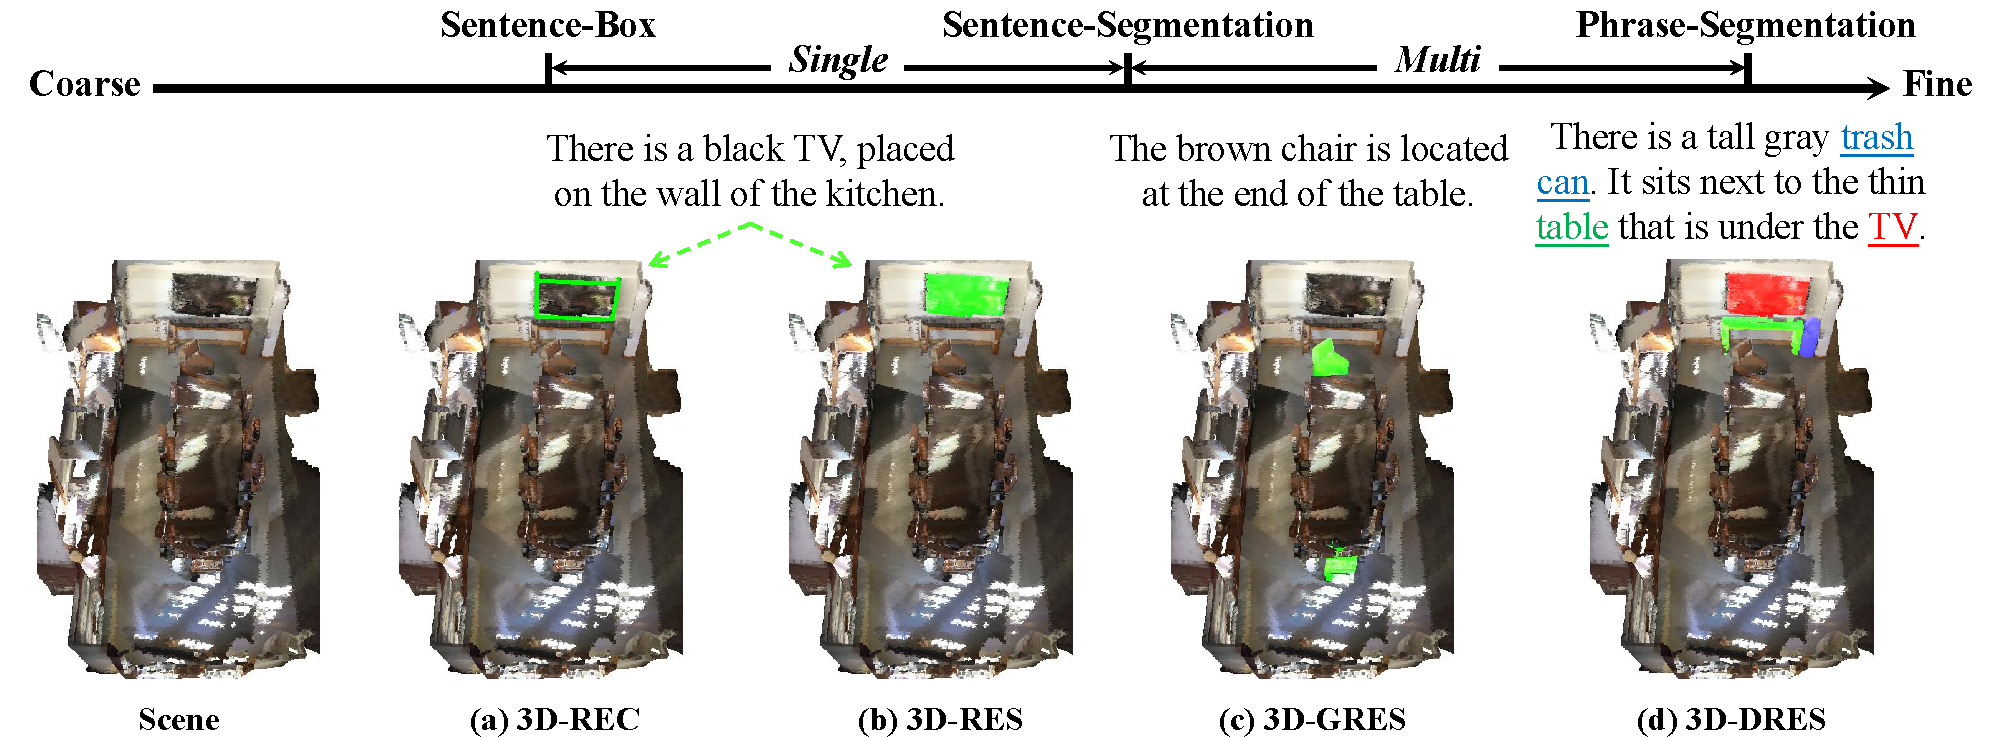
\includegraphics[width=0.98\textwidth]{Fig/fig_3D-DRES.pdf}
    \caption{3D-DRES task formulation and phrase-to-instance grounding. This placeholder should be replaced by the original task illustration comparing 3D-REC, 3D-RES, 3D-GRES, and 3D-DRES~\citep{chen3DDRESDetailed3D2026}.}
    \label{fig:extended-3ddres-placeholder}
\end{figure*}

Surprise3D shifts the evaluation from named-object grounding to spatial reasoning. It contains more than 200k vision-language pairs across more than 900 ScanNet++ scenes, more than 2.8k object classes, and more than 89k human spatial queries deliberately written without object names~\citep{huangSurprise3dDatasetSpatial2026}. This design matters because it blocks a common shortcut: if the query avoids the category name, the model cannot succeed by category recognition alone and must reason over relative position, narrative perspective, parametric perspective, or absolute distance. R$^2$S follows a similar motivation in complex 3D reasoning by identifying relevant elements before instruction processing~\citep{ningEnhancingSpatialReasoning2025}.

Open-vocabulary 3D segmentation adds another route. OV3D aligns 3D point features with contextual text features for ScanNet, Matterport3D, and nuScenes~\citep{jianglOpenvocabulary3dSemantic2024}. SAI3D builds zero-shot 3D instance segmentation from geometric primitives and multi-view SAM masks~\citep{yyinSai3dSegmentAny2024}. XMask3D uses cross-modal mask reasoning to align 3D representations with 2D-text embedding spaces~\citep{zwangXmask3dCrossmodalMask2024}. OV3D-CG then introduces contextual guidance and MLLM chain-of-thought prompting for open-vocabulary 3D instance segmentation~\citep{mzhouOV3DCGOpenvocabulary3D2025}. These works show two competing strategies: lift 2D foundation-model priors into 3D, or learn 3D-language alignment more directly. The former benefits from strong 2D models but inherits viewpoint and projection errors; the latter is geometrically cleaner but data-limited.

\subsection{Remote sensing and aerial imagery}

Remote sensing stresses both vocabulary openness and spatial precision. Objects may be small, dense, rotated, partially occluded, or visually similar across categories. Images may come from satellites, drones, RGB-thermal sensors, or different altitudes and resolutions. A category name such as ``vehicle'', ``road'', or ``building'' may correspond to very different appearances depending on scale, sensor, and viewpoint. Therefore, transferring natural-image CLIP or SAM pipelines to remote sensing often fails not because the task is exotic, but because the semantic and spatial priors are mismatched.

OVRSISBench provides a benchmark-oriented answer. It reformulates eight remote-sensing segmentation datasets under an open-vocabulary protocol, trains on DLRSD or iSAID, evaluates across target datasets with partially disjoint categories, and reports mIoU and mACC~\citep{libExploringEfficientOpenvocabulary2026}. The associated RSKT-Seg framework uses multi-directional cost-map aggregation, efficient cost-map fusion, and remote-sensing knowledge transfer, and the paper reports improvements of +3.8 mIoU and +5.9 mACC over strong baselines with faster inference. AerOSeg makes a SAM-guided version of the same argument: rotated views, domain-specific prompts, SAM-guided spatial refinement, and multi-scale decoding improve open-vocabulary segmentation on iSAID, DLRSD, and OpenEarthMap~\citep{sduttaAerosegHarnessingSam2025}. ZoRI extends the problem to zero-shot remote-sensing instance segmentation, where aerial categories have high inter-class similarity and strong intra-class variance~\citep{huangZoRIDiscriminativeZeroshot2025}.

\begin{figure}[htbp]
    \centering
    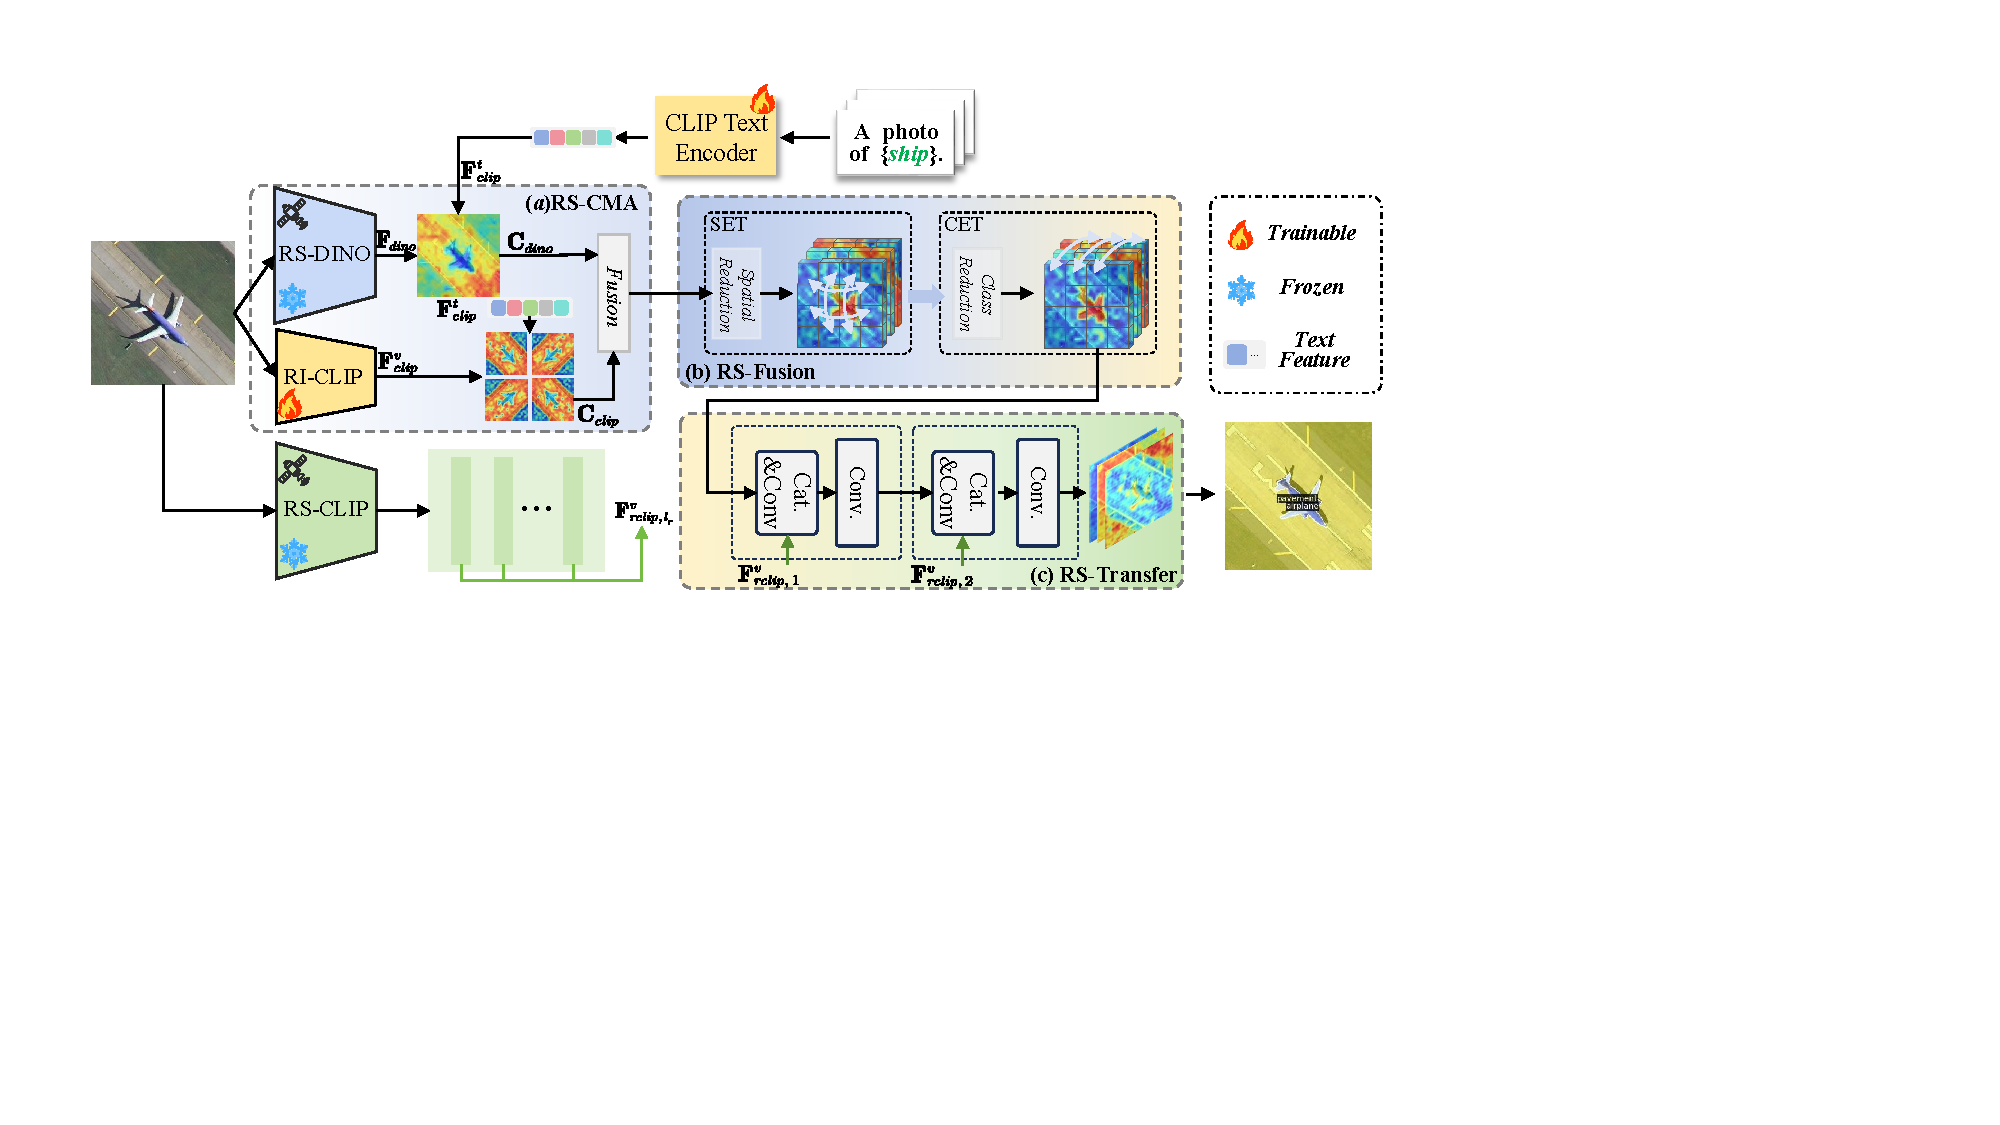
\includegraphics[width=0.98\linewidth]{Fig/fig_Exp.pdf}
    \caption{OVRSISBench and RSKT-Seg for remote-sensing open-vocabulary segmentation. This placeholder should be replaced by the original benchmark or framework figure showing the open-vocabulary dataset division, vocabulary overlap, and remote-sensing examples~\citep{libExploringEfficientOpenvocabulary2026}.}
    \label{fig:extended-ovrsis-placeholder}
\end{figure}

Referring and reasoning remote-sensing segmentation make the domain shift more explicit. RIS-LAD introduces a low-altitude drone benchmark with 13,871 image-text-mask triplets, targeting oblique viewpoints, small crowded objects, and multi-view perspectives~\citep{yeRISLADBenchmarkModel2026}. LISAt defines a language-instructed segmentation assistant for satellite imagery and trains on GRES, a geospatial reasoning segmentation dataset with 27,615 annotations across 9,205 images, plus PreGRES with over one million question-answer pairs~\citep{quenumLisatLanguageinstructedSegmentation2026}. GeoChat and FineRS further indicate that remote-sensing language interfaces require both region-level dialogue and fine-grained reasoning over small objects~\citep{kuckrejaGeochatGroundedLarge2024,zhangFineRSFinegrainedReasoning2026}. 

In summary, remote sensing is a strong test of whether open vocabulary really means open domain. A model that performs well on VOC, COCO, or ADE20K may fail under geospatial scale, rotation, and sensor shifts. Fair reporting should include training source, target datasets, class overlap, altitude or sensor domain, prompt vocabulary, and whether the method uses remote-sensing pretraining or target-domain adaptation.

\subsection{Medical, affordance, and embodied grounding}

Medical grounding changes the cost of being semantically wrong. A clinical query may be implicit, such as asking for the region relevant to a diagnostic sign rather than naming an organ explicitly. The model must interpret modality, anatomy, pathology, and clinical intent before grounding a region. MedReasoner formalizes this as Unified Medical Reasoning Grounding and introduces U-MRG-14K, which contains 14K image-mask pairs with implicit clinical queries and reasoning traces across 10 imaging modalities, 15 super-categories, and 108 categories~\citep{yanMedreasonerReinforcementLearning2026}. Its architecture decouples a clinical reasoning model from a frozen segmentation expert and uses RL rewards for format and grounding accuracy.

\begin{figure}[htbp]
    \centering
    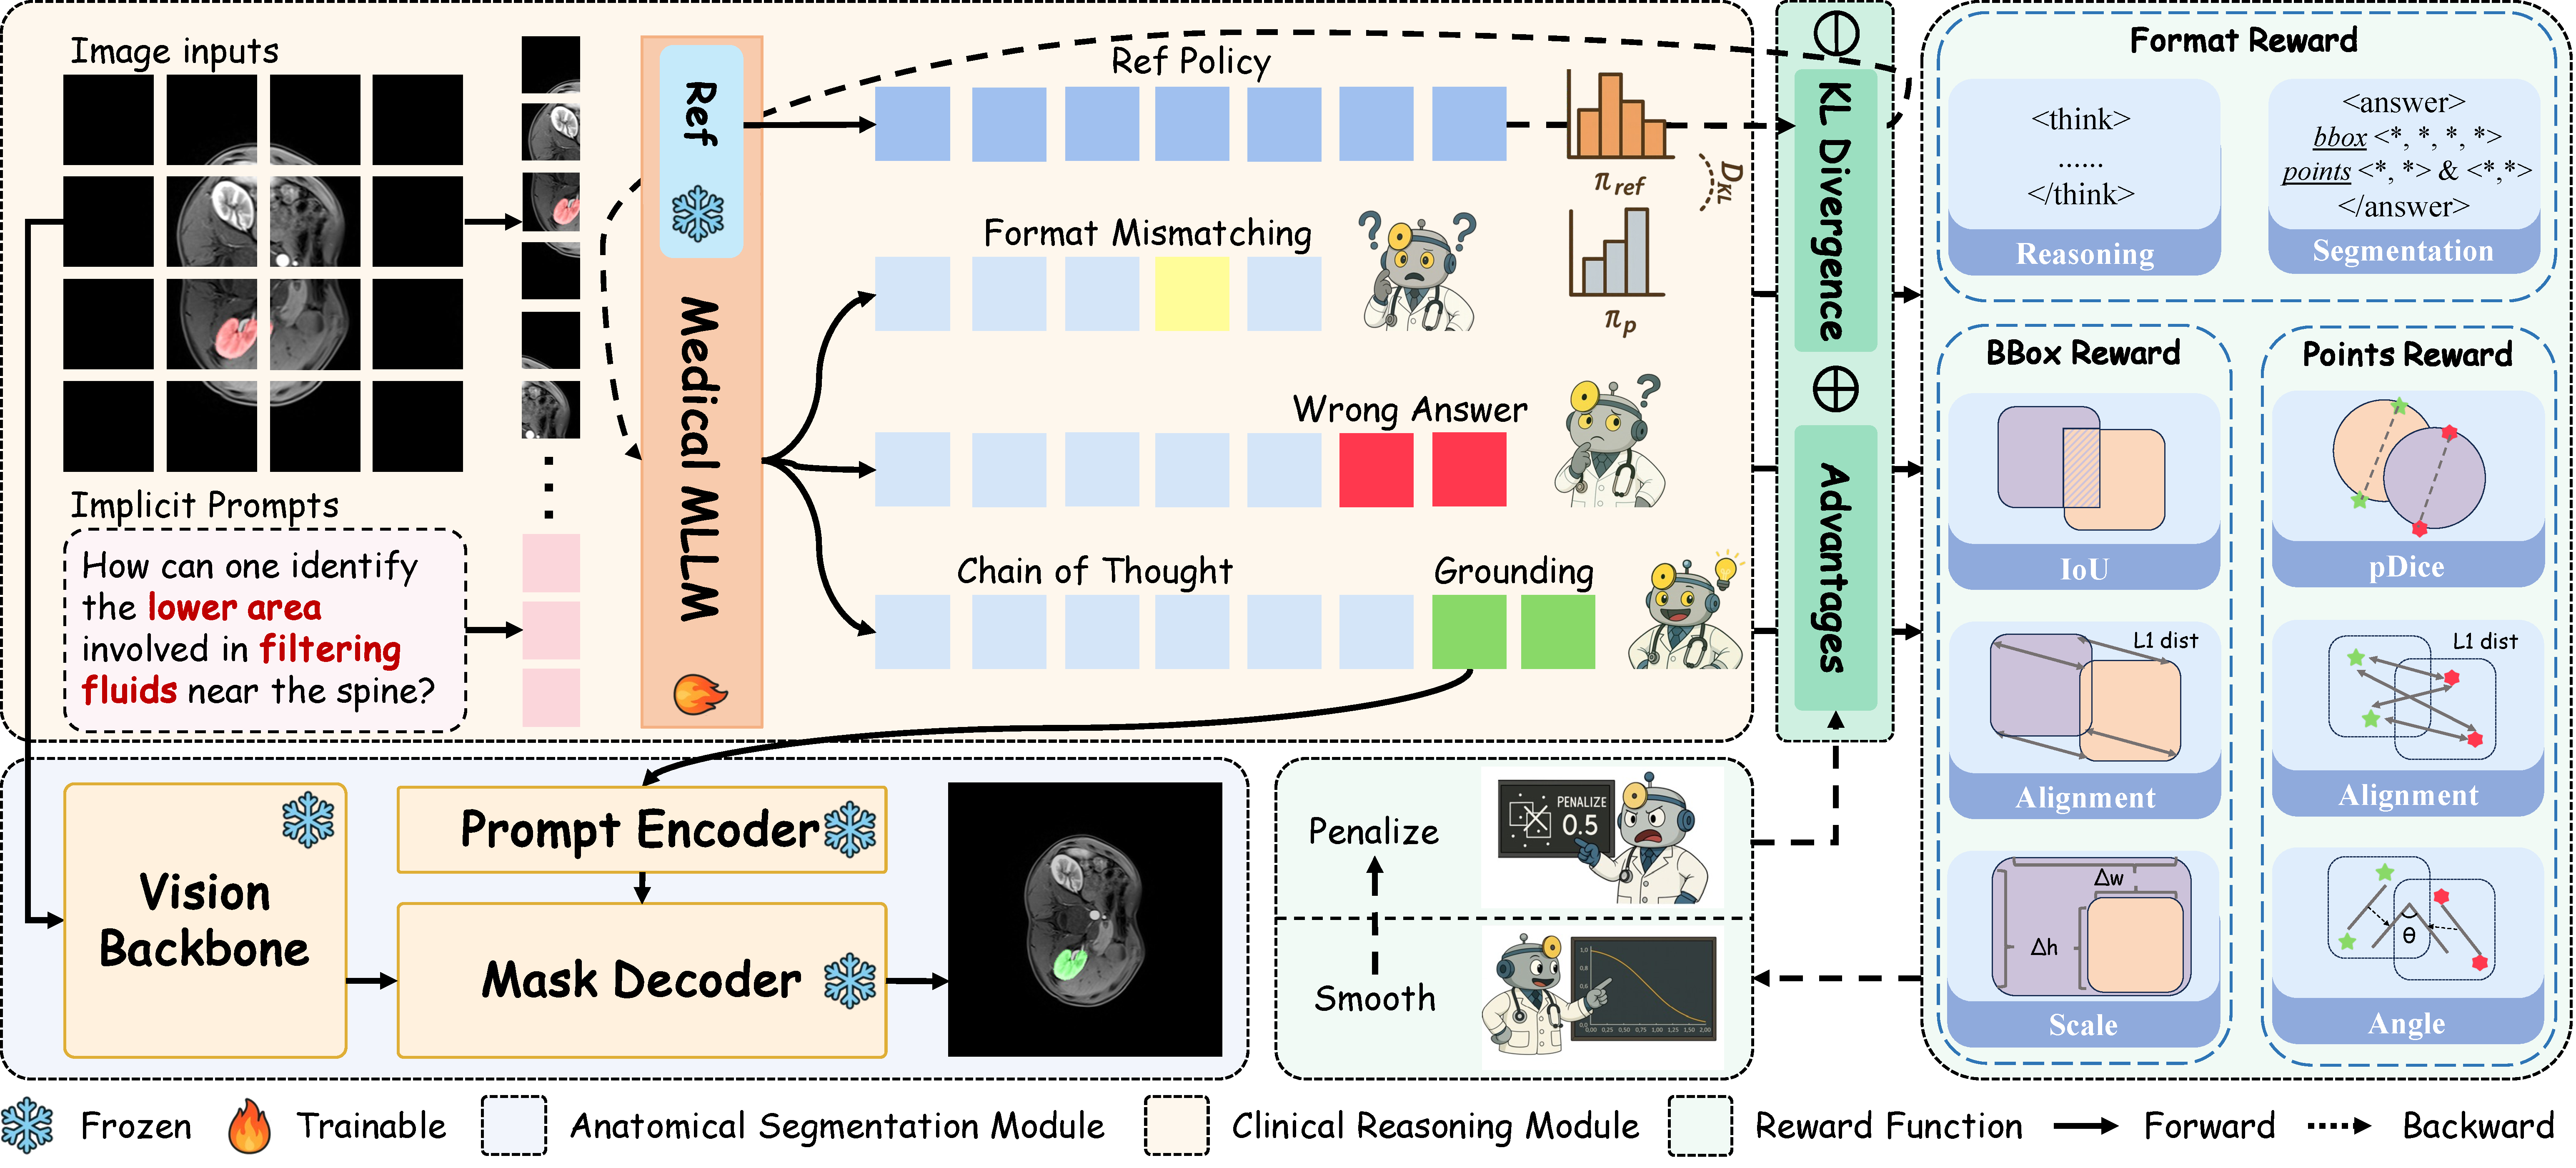
\includegraphics[width=0.98\linewidth]{Fig/fig_Med.pdf}
    \caption{MedReasoner's clinical reasoning-to-grounding pipeline. This placeholder should be replaced by the original framework figure showing how implicit clinical prompts are transformed into spatial prompts and pixel-level masks with RL rewards~\citep{yanMedreasonerReinforcementLearning2026}.}
    \label{fig:extended-medreasoner-placeholder}
\end{figure}

This medical route is closely related to pixel-grounded medical MLLMs such as MIMO, which accepts visual referring inputs and produces pixel-grounded multimodal outputs~\citep{chenMIMOMedicalVision2025}. The difference is the reasoning requirement. In ordinary medical segmentation, the label may specify the target directly. In clinical grounding, the prompt can be vague, causal, or evidence-driven. Therefore, a correct mask should be evaluated together with the reasoning trace that selected the target. Otherwise, a model could produce an anatomically plausible mask for the wrong clinical reason.

Affordance and embodied grounding shift the target from ``what object is this'' to ``where can an action be performed.'' AffordanceLLM uses vision-language knowledge to ground affordance regions for in-the-wild objects, arguing that successful affordance grounding depends on object parts, scene layout, physics, and human-object interaction knowledge~\citep{qianAffordancellmGroundingAffordance2024}. Affordance-R1 then constructs ReasonAff and optimizes affordance reasoning with GRPO using format, perception, and cognition rewards~\citep{wangAffordancer1ReinforcementLearning2026}. Its evaluation uses gIoU, cIoU, P50-95, and P50 on ReasonAff and out-of-domain AGD20K/UMD, reflecting the fact that an affordance is a part-level functional region rather than a full object mask.

Embodied systems add planning and interaction. OpenHOI connects affordance grounding with semantic task decomposition and long-horizon hand-object interaction synthesis under open-vocabulary instructions~\citep{zhangOpenhoiOpenworldHandobject2026}. Instruction-guided visual masking constructs masks for instruction-irrelevant regions so that downstream multimodal or robotic models focus on task-relevant visual content, and its IVM-Mix dataset contains one million image-instruction pairs~\citep{zhengInstructionguidedVisualMasking2024}. These works suggest that segmentation can become an intermediate control signal for action, not only an output for perception.

\subsection{Summary and discussion}

Several conclusions can be drawn from these extended scenarios. First, each scenario stresses a different hidden assumption of image-level reasoning segmentation. Videos challenge temporal identity, 3D scenes challenge viewpoint and geometry, remote sensing challenges domain and scale, medicine challenges implicit clinical semantics, and affordance grounding challenges functional part selection.

Second, the most successful designs usually preserve the core pipeline from earlier sections but add a scenario-specific reasoning layer. Video methods add frame sampling, temporal tokens, and propagation. 3D methods add multiview lifting or point-level grounding. Remote-sensing methods add rotation handling, domain prompts, and cross-dataset protocols. Medical and affordance methods add RL or explicit reasoning traces to select the correct target before segmentation.

Third, evaluation becomes more fragile as scenarios expand. A single mask metric cannot distinguish temporal drift from wrong reasoning, 2D projection errors from 3D spatial misunderstanding, label-name mismatch from remote-sensing domain failure, or object segmentation from affordance localization. Therefore, extended scenarios motivate the comparison axes in Section~\ref{sec:comparison-discussion}: semantic openness, spatial precision, training or composition cost, reasoning faithfulness, and benchmark reproducibility should be reported together rather than collapsed into one score.
